\documentclass[1p]{elsarticle_modified}
%\bibliographystyle{elsarticle-num}

%\usepackage[colorlinks]{hyperref}
%\usepackage{abbrmath_seonhwa} %\Abb, \Ascr, \Acal ,\Abf, \Afrak
\usepackage{amsfonts}
\usepackage{amssymb}
\usepackage{amsmath}
\usepackage{amsthm}
\usepackage{scalefnt}
\usepackage{amsbsy}
\usepackage{kotex}
\usepackage{caption}
\usepackage{subfig}
\usepackage{color}
\usepackage{graphicx}
\usepackage{xcolor} %% white, black, red, green, blue, cyan, magenta, yellow
\usepackage{float}
\usepackage{setspace}
\usepackage{hyperref}

\usepackage{tikz}
\usetikzlibrary{arrows}

\usepackage{multirow}
\usepackage{array} % fixed length table
\usepackage{hhline}

%%%%%%%%%%%%%%%%%%%%%
\makeatletter
\renewcommand*\env@matrix[1][\arraystretch]{%
	\edef\arraystretch{#1}%
	\hskip -\arraycolsep
	\let\@ifnextchar\new@ifnextchar
	\array{*\c@MaxMatrixCols c}}
\makeatother %https://tex.stackexchange.com/questions/14071/how-can-i-increase-the-line-spacing-in-a-matrix
%%%%%%%%%%%%%%%

\usepackage[normalem]{ulem}

\newcommand{\msout}[1]{\ifmmode\text{\sout{\ensuremath{#1}}}\else\sout{#1}\fi}
%SOURCE: \msout is \stkout macro in https://tex.stackexchange.com/questions/20609/strikeout-in-math-mode

\newcommand{\cancel}[1]{
	\ifmmode
	{\color{red}\msout{#1}}
	\else
	{\color{red}\sout{#1}}
	\fi
}

\newcommand{\add}[1]{
	{\color{blue}\uwave{#1}}
}

\newcommand{\replace}[2]{
	\ifmmode
	{\color{red}\msout{#1}}{\color{blue}\uwave{#2}}
	\else
	{\color{red}\sout{#1}}{\color{blue}\uwave{#2}}
	\fi
}

\newcommand{\Sol}{\mathcal{S}} %segment
\newcommand{\D}{D} %diagram
\newcommand{\A}{\mathcal{A}} %arc


%%%%%%%%%%%%%%%%%%%%%%%%%%%%%5 test

\def\sl{\operatorname{\textup{SL}}(2,\Cbb)}
\def\psl{\operatorname{\textup{PSL}}(2,\Cbb)}
\def\quan{\mkern 1mu \triangleright \mkern 1mu}

\theoremstyle{definition}
\newtheorem{thm}{Theorem}[section]
\newtheorem{prop}[thm]{Proposition}
\newtheorem{lem}[thm]{Lemma}
\newtheorem{ques}[thm]{Question}
\newtheorem{cor}[thm]{Corollary}
\newtheorem{defn}[thm]{Definition}
\newtheorem{exam}[thm]{Example}
\newtheorem{rmk}[thm]{Remark}
\newtheorem{alg}[thm]{Algorithm}

\newcommand{\I}{\sqrt{-1}}
\begin{document}

%\begin{frontmatter}
%
%\title{Boundary parabolic representations of knots up to 8 crossings}
%
%%% Group authors per affiliation:
%\author{Yunhi Cho} 
%\address{Department of Mathematics, University of Seoul, Seoul, Korea}
%\ead{yhcho@uos.ac.kr}
%
%
%\author{Seonhwa Kim} %\fnref{s_kim}}
%\address{Center for Geometry and Physics, Institute for Basic Science, Pohang, 37673, Korea}
%\ead{ryeona17@ibs.re.kr}
%
%\author{Hyuk Kim}
%\address{Department of Mathematical Sciences, Seoul National University, Seoul 08826, Korea}
%\ead{hyukkim@snu.ac.kr}
%
%\author{Seokbeom Yoon}
%\address{Department of Mathematical Sciences, Seoul National University, Seoul, 08826,  Korea}
%\ead{sbyoon15@snu.ac.kr}
%
%\begin{abstract}
%We find all boundary parabolic representation of knots up to 8 crossings.
%
%\end{abstract}
%\begin{keyword}
%    \MSC[2010] 57M25 
%\end{keyword}
%
%\end{frontmatter}

%\linenumbers
%\tableofcontents
%
\newcommand\colored[1]{\textcolor{white}{\rule[-0.35ex]{0.8em}{1.4ex}}\kern-0.8em\color{red} #1}%
%\newcommand\colored[1]{\textcolor{white}{ #1}\kern-2.17ex	\textcolor{white}{ #1}\kern-1.81ex	\textcolor{white}{ #1}\kern-2.15ex\color{red}#1	}

{\Large $\underline{12a_{0284}~(K12a_{0284})}$}

\setlength{\tabcolsep}{10pt}
\renewcommand{\arraystretch}{1.6}
\vspace{1cm}\begin{tabular}{m{100pt}>{\centering\arraybackslash}m{274pt}}
\multirow{5}{120pt}{
	\centering
	\includegraphics[width=112pt]{../../../GIT/diagram.site/Diagrams/png/1085_12a_0284.png}\\
\ \ \ A knot diagram\footnotemark}&
\allowdisplaybreaks
\textbf{Linearized knot diagam} \\
\cline{2-2}
 &
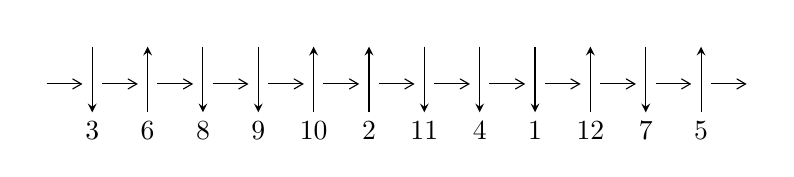
\begin{tikzpicture}[x=20pt, y=17pt]
	% nodes
	\node (C0) at (0, 0) {};
	\node (C1) at (1, 0) {};
	\node (C1U) at (1, +1) {};
	\node (C1D) at (1, -1) {3};

	\node (C2) at (2, 0) {};
	\node (C2U) at (2, +1) {};
	\node (C2D) at (2, -1) {6};

	\node (C3) at (3, 0) {};
	\node (C3U) at (3, +1) {};
	\node (C3D) at (3, -1) {8};

	\node (C4) at (4, 0) {};
	\node (C4U) at (4, +1) {};
	\node (C4D) at (4, -1) {9};

	\node (C5) at (5, 0) {};
	\node (C5U) at (5, +1) {};
	\node (C5D) at (5, -1) {10};

	\node (C6) at (6, 0) {};
	\node (C6U) at (6, +1) {};
	\node (C6D) at (6, -1) {2};

	\node (C7) at (7, 0) {};
	\node (C7U) at (7, +1) {};
	\node (C7D) at (7, -1) {11};

	\node (C8) at (8, 0) {};
	\node (C8U) at (8, +1) {};
	\node (C8D) at (8, -1) {4};

	\node (C9) at (9, 0) {};
	\node (C9U) at (9, +1) {};
	\node (C9D) at (9, -1) {1};

	\node (C10) at (10, 0) {};
	\node (C10U) at (10, +1) {};
	\node (C10D) at (10, -1) {12};

	\node (C11) at (11, 0) {};
	\node (C11U) at (11, +1) {};
	\node (C11D) at (11, -1) {7};

	\node (C12) at (12, 0) {};
	\node (C12U) at (12, +1) {};
	\node (C12D) at (12, -1) {5};
	\node (C13) at (13, 0) {};

	% arrows
	\draw[->,>={angle 60}]
	(C0) edge (C1) (C1) edge (C2) (C2) edge (C3) (C3) edge (C4) (C4) edge (C5) (C5) edge (C6) (C6) edge (C7) (C7) edge (C8) (C8) edge (C9) (C9) edge (C10) (C10) edge (C11) (C11) edge (C12) (C12) edge (C13) ;	\draw[->,>=stealth]
	(C1U) edge (C1D) (C2D) edge (C2U) (C3U) edge (C3D) (C4U) edge (C4D) (C5D) edge (C5U) (C6D) edge (C6U) (C7U) edge (C7D) (C8U) edge (C8D) (C9U) edge (C9D) (C10D) edge (C10U) (C11U) edge (C11D) (C12D) edge (C12U) ;
	\end{tikzpicture} \\
\hhline{~~} \\& 
\textbf{Solving Sequence} \\ \cline{2-2} 
 &
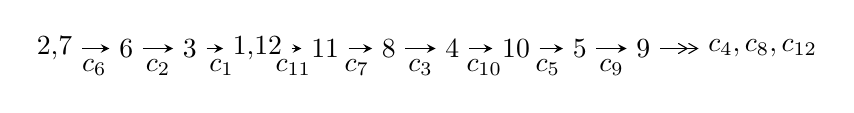
\begin{tikzpicture}[x=23pt, y=7pt]
	% node
	\node (A0) at (-1/8, 0) {2,7};
	\node (A1) at (1, 0) {6};
	\node (A2) at (2, 0) {3};
	\node (A3) at (49/16, 0) {1,12};
	\node (A4) at (33/8, 0) {11};
	\node (A5) at (41/8, 0) {8};
	\node (A6) at (49/8, 0) {4};
	\node (A7) at (57/8, 0) {10};
	\node (A8) at (65/8, 0) {5};
	\node (A9) at (73/8, 0) {9};
	\node (C1) at (1/2, -1) {$c_{6}$};
	\node (C2) at (3/2, -1) {$c_{2}$};
	\node (C3) at (5/2, -1) {$c_{1}$};
	\node (C4) at (29/8, -1) {$c_{11}$};
	\node (C5) at (37/8, -1) {$c_{7}$};
	\node (C6) at (45/8, -1) {$c_{3}$};
	\node (C7) at (53/8, -1) {$c_{10}$};
	\node (C8) at (61/8, -1) {$c_{5}$};
	\node (C9) at (69/8, -1) {$c_{9}$};
	\node (A10) at (11, 0) {$c_{4},c_{8},c_{12}$};

	% edge
	\draw[->,>=stealth]	
	(A0) edge (A1) (A1) edge (A2) (A2) edge (A3) (A3) edge (A4) (A4) edge (A5) (A5) edge (A6) (A6) edge (A7) (A7) edge (A8) (A8) edge (A9) ;
	\draw[->>,>={angle 60}]	
	(A9) edge (A10);
\end{tikzpicture} \\ 

\end{tabular} \\

\footnotetext{
The image of knot diagram is generated by the software ``\textbf{Draw programme}" developed by Andrew Bartholomew(\url{http://www.layer8.co.uk/maths/draw/index.htm\#Running-draw}), where we modified some parts for our purpose(\url{https://github.com/CATsTAILs/LinksPainter}).
}\phantom \\ \newline 
\centering \textbf{Ideals for irreducible components\footnotemark of $X_{\text{par}}$} 
 
\begin{align*}
I^u_{1}&=\langle 
2.11523\times10^{322} u^{128}-5.51615\times10^{322} u^{127}+\cdots+7.53841\times10^{322} b+8.81896\times10^{322},\\
\phantom{I^u_{1}}&\phantom{= \langle  }-2.42099\times10^{324} u^{128}+1.88050\times10^{324} u^{127}+\cdots+4.89997\times10^{324} a-4.91206\times10^{324},\\
\phantom{I^u_{1}}&\phantom{= \langle  }u^{129}- u^{128}+\cdots+137 u-13\rangle \\
I^u_{2}&=\langle 
5 u^{27}+6 u^{26}+\cdots+b+2,\;6 u^{27}+19 u^{26}+\cdots+a+23,\;u^{28}+2 u^{27}+\cdots+2 u+1\rangle \\
\\
\end{align*}
\raggedright * 2 irreducible components of $\dim_{\mathbb{C}}=0$, with total 157 representations.\\
\footnotetext{All coefficients of polynomials are rational numbers. But the coefficients are sometimes approximated in decimal forms when there is not enough margin.}
\newpage
\renewcommand{\arraystretch}{1}
\centering \section*{I. $I^u_{1}= \langle 2.12\times10^{322} u^{128}-5.52\times10^{322} u^{127}+\cdots+7.54\times10^{322} b+8.82\times10^{322},\;-2.42\times10^{324} u^{128}+1.88\times10^{324} u^{127}+\cdots+4.90\times10^{324} a-4.91\times10^{324},\;u^{129}- u^{128}+\cdots+137 u-13 \rangle$}
\flushleft \textbf{(i) Arc colorings}\\
\begin{tabular}{m{7pt} m{180pt} m{7pt} m{180pt} }
\flushright $a_{2}=$&$\begin{pmatrix}0\\u\end{pmatrix}$ \\
\flushright $a_{7}=$&$\begin{pmatrix}1\\0\end{pmatrix}$ \\
\flushright $a_{6}=$&$\begin{pmatrix}1\\u^2\end{pmatrix}$ \\
\flushright $a_{3}=$&$\begin{pmatrix}u\\u^3+u\end{pmatrix}$ \\
\flushright $a_{1}=$&$\begin{pmatrix}u^3\\u^5+u^3+u\end{pmatrix}$ \\
\flushright $a_{12}=$&$\begin{pmatrix}0.494084 u^{128}-0.383778 u^{127}+\cdots-6.96403 u+1.00247\\-0.280594 u^{128}+0.731739 u^{127}+\cdots+27.8062 u-1.16987\end{pmatrix}$ \\
\flushright $a_{11}=$&$\begin{pmatrix}0.213490 u^{128}+0.347960 u^{127}+\cdots+20.8422 u-0.167402\\-0.280594 u^{128}+0.731739 u^{127}+\cdots+27.8062 u-1.16987\end{pmatrix}$ \\
\flushright $a_{8}=$&$\begin{pmatrix}-1.40665 u^{128}+1.42022 u^{127}+\cdots-26.1537 u+0.0735769\\0.569437 u^{128}-1.35911 u^{127}+\cdots-107.757 u+8.46868\end{pmatrix}$ \\
\flushright $a_{4}=$&$\begin{pmatrix}0.207779 u^{128}-0.290200 u^{127}+\cdots-63.9032 u+4.81670\\0.559337 u^{128}-0.771287 u^{127}+\cdots-22.2391 u+1.72665\end{pmatrix}$ \\
\flushright $a_{10}=$&$\begin{pmatrix}1.39925 u^{128}-2.13313 u^{127}+\cdots+27.0446 u-7.75958\\-0.717274 u^{128}+1.61861 u^{127}+\cdots+79.7326 u-7.23816\end{pmatrix}$ \\
\flushright $a_{5}=$&$\begin{pmatrix}-0.499032 u^{128}+0.282170 u^{127}+\cdots-26.1238 u+5.09116\\0.435156 u^{128}-0.835389 u^{127}+\cdots-28.2553 u+1.29870\end{pmatrix}$ \\
\flushright $a_{9}=$&$\begin{pmatrix}1.09787 u^{128}-1.38838 u^{127}+\cdots+56.8709 u-9.95927\\-0.435694 u^{128}+1.08524 u^{127}+\cdots+67.5703 u-6.43747\end{pmatrix}$\\&\end{tabular}
\flushleft \textbf{(ii) Obstruction class $= -1$}\\~\\
\flushleft \textbf{(iii) Cusp Shapes $= 5.38288 u^{128}-6.93878 u^{127}+\cdots-56.7921 u-2.13704$}\\~\\
\newpage\renewcommand{\arraystretch}{1}
\flushleft \textbf{(iv) u-Polynomials at the component}\newline \\
\begin{tabular}{m{50pt}|m{274pt}}
Crossings & \hspace{64pt}u-Polynomials at each crossing \\
\hline $$\begin{aligned}c_{1}\end{aligned}$$&$\begin{aligned}
&u^{129}+61 u^{128}+\cdots+2857 u-169
\end{aligned}$\\
\hline $$\begin{aligned}c_{2},c_{6}\end{aligned}$$&$\begin{aligned}
&u^{129}+u^{128}+\cdots+137 u+13
\end{aligned}$\\
\hline $$\begin{aligned}c_{3},c_{4},c_{8}\end{aligned}$$&$\begin{aligned}
&u^{129}- u^{128}+\cdots-35 u+1
\end{aligned}$\\
\hline $$\begin{aligned}c_{5}\end{aligned}$$&$\begin{aligned}
&u^{129}+u^{128}+\cdots-17 u+3
\end{aligned}$\\
\hline $$\begin{aligned}c_{7},c_{11}\end{aligned}$$&$\begin{aligned}
&u^{129}- u^{128}+\cdots+1041 u+391
\end{aligned}$\\
\hline $$\begin{aligned}c_{9}\end{aligned}$$&$\begin{aligned}
&u^{129}-11 u^{128}+\cdots-2772 u-1336
\end{aligned}$\\
\hline $$\begin{aligned}c_{10}\end{aligned}$$&$\begin{aligned}
&u^{129}-53 u^{128}+\cdots-3530901 u+152881
\end{aligned}$\\
\hline $$\begin{aligned}c_{12}\end{aligned}$$&$\begin{aligned}
&u^{129}-5 u^{128}+\cdots+87185 u+62623
\end{aligned}$\\
\hline
\end{tabular}\\~\\
\newpage\renewcommand{\arraystretch}{1}
\flushleft \textbf{(v) Riley Polynomials at the component}\newline \\
\begin{tabular}{m{50pt}|m{274pt}}
Crossings & \hspace{64pt}Riley Polynomials at each crossing \\
\hline $$\begin{aligned}c_{1}\end{aligned}$$&$\begin{aligned}
&y^{129}+29 y^{128}+\cdots+4737157 y-28561
\end{aligned}$\\
\hline $$\begin{aligned}c_{2},c_{6}\end{aligned}$$&$\begin{aligned}
&y^{129}+61 y^{128}+\cdots+2857 y-169
\end{aligned}$\\
\hline $$\begin{aligned}c_{3},c_{4},c_{8}\end{aligned}$$&$\begin{aligned}
&y^{129}-131 y^{128}+\cdots+111 y-1
\end{aligned}$\\
\hline $$\begin{aligned}c_{5}\end{aligned}$$&$\begin{aligned}
&y^{129}+9 y^{128}+\cdots-293 y-9
\end{aligned}$\\
\hline $$\begin{aligned}c_{7},c_{11}\end{aligned}$$&$\begin{aligned}
&y^{129}+53 y^{128}+\cdots-3530901 y-152881
\end{aligned}$\\
\hline $$\begin{aligned}c_{9}\end{aligned}$$&$\begin{aligned}
&y^{129}-25 y^{128}+\cdots+84295568 y-1784896
\end{aligned}$\\
\hline $$\begin{aligned}c_{10}\end{aligned}$$&$\begin{aligned}
&y^{129}+61 y^{128}+\cdots+863028617863 y-23372600161
\end{aligned}$\\
\hline $$\begin{aligned}c_{12}\end{aligned}$$&$\begin{aligned}
&y^{129}+47 y^{128}+\cdots-202889332557 y-3921640129
\end{aligned}$\\
\hline
\end{tabular}\\~\\
\newpage\flushleft \textbf{(vi) Complex Volumes and Cusp Shapes}
$$\begin{array}{c|c|c}  
\text{Solutions to }I^u_{1}& \I (\text{vol} + \sqrt{-1}CS) & \text{Cusp shape}\\
 \hline 
\begin{aligned}
u &= -0.225214 + 0.970442 I \\
a &= \phantom{-}0.188196 - 0.699549 I \\
b &= \phantom{-}0.069903 + 0.599101 I\end{aligned}
 & -0.80326 - 1.93442 I & \phantom{-0.000000 } 0 \\ \hline\begin{aligned}
u &= -0.225214 - 0.970442 I \\
a &= \phantom{-}0.188196 + 0.699549 I \\
b &= \phantom{-}0.069903 - 0.599101 I\end{aligned}
 & -0.80326 + 1.93442 I & \phantom{-0.000000 } 0 \\ \hline\begin{aligned}
u &= \phantom{-}0.328434 + 0.950935 I \\
a &= \phantom{-}0.29600 - 1.84878 I \\
b &= -0.227836 - 0.965332 I\end{aligned}
 & -5.38486 + 3.82100 I & \phantom{-0.000000 } 0 \\ \hline\begin{aligned}
u &= \phantom{-}0.328434 - 0.950935 I \\
a &= \phantom{-}0.29600 + 1.84878 I \\
b &= -0.227836 + 0.965332 I\end{aligned}
 & -5.38486 - 3.82100 I & \phantom{-0.000000 } 0 \\ \hline\begin{aligned}
u &= \phantom{-}0.362252 + 0.943135 I \\
a &= -0.719526 - 1.108760 I \\
b &= \phantom{-}0.727767 + 0.830631 I\end{aligned}
 & -1.81178 - 0.98745 I & \phantom{-0.000000 } 0 \\ \hline\begin{aligned}
u &= \phantom{-}0.362252 - 0.943135 I \\
a &= -0.719526 + 1.108760 I \\
b &= \phantom{-}0.727767 - 0.830631 I\end{aligned}
 & -1.81178 + 0.98745 I & \phantom{-0.000000 } 0 \\ \hline\begin{aligned}
u &= \phantom{-}0.999843 + 0.147388 I \\
a &= -0.967711 - 0.726256 I \\
b &= \phantom{-}0.419979 - 1.062220 I\end{aligned}
 & -0.21128 + 3.47728 I & \phantom{-0.000000 } 0 \\ \hline\begin{aligned}
u &= \phantom{-}0.999843 - 0.147388 I \\
a &= -0.967711 + 0.726256 I \\
b &= \phantom{-}0.419979 + 1.062220 I\end{aligned}
 & -0.21128 - 3.47728 I & \phantom{-0.000000 } 0 \\ \hline\begin{aligned}
u &= -0.940780 + 0.295046 I \\
a &= -0.571993 + 0.318063 I \\
b &= \phantom{-}0.899065 + 0.496812 I\end{aligned}
 & -6.84068 + 6.76676 I & \phantom{-0.000000 } 0 \\ \hline\begin{aligned}
u &= -0.940780 - 0.295046 I \\
a &= -0.571993 - 0.318063 I \\
b &= \phantom{-}0.899065 - 0.496812 I\end{aligned}
 & -6.84068 - 6.76676 I & \phantom{-0.000000 } 0\\
 \hline 
 \end{array}$$\newpage$$\begin{array}{c|c|c}  
\text{Solutions to }I^u_{1}& \I (\text{vol} + \sqrt{-1}CS) & \text{Cusp shape}\\
 \hline 
\begin{aligned}
u &= -0.705773 + 0.739442 I \\
a &= -0.286635 + 0.922999 I \\
b &= \phantom{-}0.176137 + 1.016140 I\end{aligned}
 & \phantom{-}3.36266 - 2.76080 I & \phantom{-0.000000 } 0 \\ \hline\begin{aligned}
u &= -0.705773 - 0.739442 I \\
a &= -0.286635 - 0.922999 I \\
b &= \phantom{-}0.176137 - 1.016140 I\end{aligned}
 & \phantom{-}3.36266 + 2.76080 I & \phantom{-0.000000 } 0 \\ \hline\begin{aligned}
u &= -0.329913 + 0.971134 I \\
a &= -0.343444 + 0.272427 I \\
b &= -0.383042 + 1.321060 I\end{aligned}
 & -3.86381 + 3.18454 I & \phantom{-0.000000 } 0 \\ \hline\begin{aligned}
u &= -0.329913 - 0.971134 I \\
a &= -0.343444 - 0.272427 I \\
b &= -0.383042 - 1.321060 I\end{aligned}
 & -3.86381 - 3.18454 I & \phantom{-0.000000 } 0 \\ \hline\begin{aligned}
u &= \phantom{-}0.351334 + 0.972584 I \\
a &= -0.787019 - 1.148740 I \\
b &= \phantom{-}0.899896 + 0.284403 I\end{aligned}
 & -3.37868 + 1.16334 I & \phantom{-0.000000 } 0 \\ \hline\begin{aligned}
u &= \phantom{-}0.351334 - 0.972584 I \\
a &= -0.787019 + 1.148740 I \\
b &= \phantom{-}0.899896 - 0.284403 I\end{aligned}
 & -3.37868 - 1.16334 I & \phantom{-0.000000 } 0 \\ \hline\begin{aligned}
u &= \phantom{-}0.714434 + 0.645186 I \\
a &= \phantom{-}0.772470 + 0.761469 I \\
b &= -0.081513 + 1.176680 I\end{aligned}
 & \phantom{-}5.07712 - 1.16370 I & \phantom{-0.000000 } 0 \\ \hline\begin{aligned}
u &= \phantom{-}0.714434 - 0.645186 I \\
a &= \phantom{-}0.772470 - 0.761469 I \\
b &= -0.081513 - 1.176680 I\end{aligned}
 & \phantom{-}5.07712 + 1.16370 I & \phantom{-0.000000 } 0 \\ \hline\begin{aligned}
u &= -0.231944 + 0.924569 I \\
a &= \phantom{-}3.02381 + 0.36742 I \\
b &= -0.523114 - 1.102980 I\end{aligned}
 & -3.44731 - 5.48846 I & \phantom{-0.000000 } 0 \\ \hline\begin{aligned}
u &= -0.231944 - 0.924569 I \\
a &= \phantom{-}3.02381 - 0.36742 I \\
b &= -0.523114 + 1.102980 I\end{aligned}
 & -3.44731 + 5.48846 I & \phantom{-0.000000 } 0\\
 \hline 
 \end{array}$$\newpage$$\begin{array}{c|c|c}  
\text{Solutions to }I^u_{1}& \I (\text{vol} + \sqrt{-1}CS) & \text{Cusp shape}\\
 \hline 
\begin{aligned}
u &= \phantom{-}0.258325 + 1.017820 I \\
a &= \phantom{-}1.73059 + 0.81158 I \\
b &= -0.824534 - 0.944981 I\end{aligned}
 & -10.21390 - 2.58554 I & \phantom{-0.000000 } 0 \\ \hline\begin{aligned}
u &= \phantom{-}0.258325 - 1.017820 I \\
a &= \phantom{-}1.73059 - 0.81158 I \\
b &= -0.824534 + 0.944981 I\end{aligned}
 & -10.21390 + 2.58554 I & \phantom{-0.000000 } 0 \\ \hline\begin{aligned}
u &= \phantom{-}0.858414 + 0.395936 I \\
a &= \phantom{-}0.745540 - 0.381485 I \\
b &= -0.627590 - 1.085720 I\end{aligned}
 & \phantom{-}1.49834 - 8.61565 I & \phantom{-0.000000 } 0 \\ \hline\begin{aligned}
u &= \phantom{-}0.858414 - 0.395936 I \\
a &= \phantom{-}0.745540 + 0.381485 I \\
b &= -0.627590 + 1.085720 I\end{aligned}
 & \phantom{-}1.49834 + 8.61565 I & \phantom{-0.000000 } 0 \\ \hline\begin{aligned}
u &= \phantom{-}0.916613 + 0.546470 I \\
a &= -0.821334 - 0.095251 I \\
b &= \phantom{-}0.365381 + 0.906065 I\end{aligned}
 & -1.12063 + 1.21435 I & \phantom{-0.000000 } 0 \\ \hline\begin{aligned}
u &= \phantom{-}0.916613 - 0.546470 I \\
a &= -0.821334 + 0.095251 I \\
b &= \phantom{-}0.365381 - 0.906065 I\end{aligned}
 & -1.12063 - 1.21435 I & \phantom{-0.000000 } 0 \\ \hline\begin{aligned}
u &= -0.747457 + 0.557539 I \\
a &= -0.203435 + 0.454510 I \\
b &= -0.696615 + 1.158500 I\end{aligned}
 & -4.76573 + 3.31723 I & \phantom{-0.000000 } 0 \\ \hline\begin{aligned}
u &= -0.747457 - 0.557539 I \\
a &= -0.203435 - 0.454510 I \\
b &= -0.696615 - 1.158500 I\end{aligned}
 & -4.76573 - 3.31723 I & \phantom{-0.000000 } 0 \\ \hline\begin{aligned}
u &= \phantom{-}0.239028 + 0.900459 I \\
a &= \phantom{-}3.30663 - 0.84537 I \\
b &= -0.479176 + 0.702293 I\end{aligned}
 & -5.03356 - 1.35646 I & \phantom{-0.000000 } 0 \\ \hline\begin{aligned}
u &= \phantom{-}0.239028 - 0.900459 I \\
a &= \phantom{-}3.30663 + 0.84537 I \\
b &= -0.479176 - 0.702293 I\end{aligned}
 & -5.03356 + 1.35646 I & \phantom{-0.000000 } 0\\
 \hline 
 \end{array}$$\newpage$$\begin{array}{c|c|c}  
\text{Solutions to }I^u_{1}& \I (\text{vol} + \sqrt{-1}CS) & \text{Cusp shape}\\
 \hline 
\begin{aligned}
u &= -0.240069 + 0.895280 I \\
a &= \phantom{-}1.00002 - 1.53176 I \\
b &= -1.05559 + 1.02499 I\end{aligned}
 & -9.15850 + 2.76252 I & \phantom{-0.000000 } 0 \\ \hline\begin{aligned}
u &= -0.240069 - 0.895280 I \\
a &= \phantom{-}1.00002 + 1.53176 I \\
b &= -1.05559 - 1.02499 I\end{aligned}
 & -9.15850 - 2.76252 I & \phantom{-0.000000 } 0 \\ \hline\begin{aligned}
u &= \phantom{-}0.089015 + 1.069970 I \\
a &= \phantom{-}2.00501 - 0.82963 I \\
b &= -0.642587 + 0.590143 I\end{aligned}
 & -5.03807 - 1.18501 I & \phantom{-0.000000 } 0 \\ \hline\begin{aligned}
u &= \phantom{-}0.089015 - 1.069970 I \\
a &= \phantom{-}2.00501 + 0.82963 I \\
b &= -0.642587 - 0.590143 I\end{aligned}
 & -5.03807 + 1.18501 I & \phantom{-0.000000 } 0 \\ \hline\begin{aligned}
u &= \phantom{-}0.558403 + 0.926828 I \\
a &= -1.76060 - 0.08232 I \\
b &= \phantom{-}0.675429 - 0.608453 I\end{aligned}
 & -2.19993 + 4.47085 I & \phantom{-0.000000 } 0 \\ \hline\begin{aligned}
u &= \phantom{-}0.558403 - 0.926828 I \\
a &= -1.76060 + 0.08232 I \\
b &= \phantom{-}0.675429 + 0.608453 I\end{aligned}
 & -2.19993 - 4.47085 I & \phantom{-0.000000 } 0 \\ \hline\begin{aligned}
u &= -0.871691 + 0.260471 I \\
a &= \phantom{-}0.741627 + 0.383723 I \\
b &= -0.411096 + 0.971805 I\end{aligned}
 & \phantom{-}3.01496 + 1.37794 I & \phantom{-0.000000 } 0 \\ \hline\begin{aligned}
u &= -0.871691 - 0.260471 I \\
a &= \phantom{-}0.741627 - 0.383723 I \\
b &= -0.411096 - 0.971805 I\end{aligned}
 & \phantom{-}3.01496 - 1.37794 I & \phantom{-0.000000 } 0 \\ \hline\begin{aligned}
u &= -1.025460 + 0.377398 I \\
a &= -0.564098 - 0.438983 I \\
b &= \phantom{-}0.678901 - 1.117400 I\end{aligned}
 & -4.95449 + 12.58240 I & \phantom{-0.000000 } 0 \\ \hline\begin{aligned}
u &= -1.025460 - 0.377398 I \\
a &= -0.564098 + 0.438983 I \\
b &= \phantom{-}0.678901 + 1.117400 I\end{aligned}
 & -4.95449 - 12.58240 I & \phantom{-0.000000 } 0\\
 \hline 
 \end{array}$$\newpage$$\begin{array}{c|c|c}  
\text{Solutions to }I^u_{1}& \I (\text{vol} + \sqrt{-1}CS) & \text{Cusp shape}\\
 \hline 
\begin{aligned}
u &= -0.374909 + 1.031730 I \\
a &= \phantom{-}1.81385 - 0.23953 I \\
b &= -1.219110 - 0.707738 I\end{aligned}
 & -10.09170 - 5.09552 I & \phantom{-0.000000 } 0 \\ \hline\begin{aligned}
u &= -0.374909 - 1.031730 I \\
a &= \phantom{-}1.81385 + 0.23953 I \\
b &= -1.219110 + 0.707738 I\end{aligned}
 & -10.09170 + 5.09552 I & \phantom{-0.000000 } 0 \\ \hline\begin{aligned}
u &= -0.469964 + 1.009150 I \\
a &= -2.75594 + 0.93516 I \\
b &= \phantom{-}0.571142 + 0.885822 I\end{aligned}
 & -2.13464 - 3.79367 I & \phantom{-0.000000 } 0 \\ \hline\begin{aligned}
u &= -0.469964 - 1.009150 I \\
a &= -2.75594 - 0.93516 I \\
b &= \phantom{-}0.571142 - 0.885822 I\end{aligned}
 & -2.13464 + 3.79367 I & \phantom{-0.000000 } 0 \\ \hline\begin{aligned}
u &= -0.459458 + 1.015260 I \\
a &= -1.25021 + 1.52465 I \\
b &= \phantom{-}0.764541 - 0.702431 I\end{aligned}
 & -2.18902 - 2.29239 I & \phantom{-0.000000 } 0 \\ \hline\begin{aligned}
u &= -0.459458 - 1.015260 I \\
a &= -1.25021 - 1.52465 I \\
b &= \phantom{-}0.764541 + 0.702431 I\end{aligned}
 & -2.18902 + 2.29239 I & \phantom{-0.000000 } 0 \\ \hline\begin{aligned}
u &= \phantom{-}0.617454 + 0.927981 I \\
a &= -1.83805 - 0.02741 I \\
b &= \phantom{-}0.573735 - 0.659494 I\end{aligned}
 & -2.20423 + 4.46264 I & \phantom{-0.000000 } 0 \\ \hline\begin{aligned}
u &= \phantom{-}0.617454 - 0.927981 I \\
a &= -1.83805 + 0.02741 I \\
b &= \phantom{-}0.573735 + 0.659494 I\end{aligned}
 & -2.20423 - 4.46264 I & \phantom{-0.000000 } 0 \\ \hline\begin{aligned}
u &= -0.902145 + 0.678839 I \\
a &= \phantom{-}0.968996 - 0.567142 I \\
b &= -0.427319 - 0.991107 I\end{aligned}
 & \phantom{-}2.92976 - 4.56971 I & \phantom{-0.000000 } 0 \\ \hline\begin{aligned}
u &= -0.902145 - 0.678839 I \\
a &= \phantom{-}0.968996 + 0.567142 I \\
b &= -0.427319 + 0.991107 I\end{aligned}
 & \phantom{-}2.92976 + 4.56971 I & \phantom{-0.000000 } 0\\
 \hline 
 \end{array}$$\newpage$$\begin{array}{c|c|c}  
\text{Solutions to }I^u_{1}& \I (\text{vol} + \sqrt{-1}CS) & \text{Cusp shape}\\
 \hline 
\begin{aligned}
u &= \phantom{-}0.866221\phantom{ +0.000000I} \\
a &= -0.446291\phantom{ +0.000000I} \\
b &= \phantom{-}0.555077\phantom{ +0.000000I}\end{aligned}
 & -2.96518\phantom{ +0.000000I} & \phantom{-0.000000 } 0 \\ \hline\begin{aligned}
u &= -0.361536 + 1.077970 I \\
a &= -0.52789 + 1.89034 I \\
b &= \phantom{-}0.570408 - 0.819470 I\end{aligned}
 & -2.34980 + 0.75723 I & \phantom{-0.000000 } 0 \\ \hline\begin{aligned}
u &= -0.361536 - 1.077970 I \\
a &= -0.52789 - 1.89034 I \\
b &= \phantom{-}0.570408 + 0.819470 I\end{aligned}
 & -2.34980 - 0.75723 I & \phantom{-0.000000 } 0 \\ \hline\begin{aligned}
u &= \phantom{-}0.509217 + 1.017550 I \\
a &= -2.17381 - 0.47768 I \\
b &= \phantom{-}0.667686 - 1.174370 I\end{aligned}
 & -0.79292 + 6.94260 I & \phantom{-0.000000 } 0 \\ \hline\begin{aligned}
u &= \phantom{-}0.509217 - 1.017550 I \\
a &= -2.17381 + 0.47768 I \\
b &= \phantom{-}0.667686 + 1.174370 I\end{aligned}
 & -0.79292 - 6.94260 I & \phantom{-0.000000 } 0 \\ \hline\begin{aligned}
u &= -0.691403 + 0.514811 I \\
a &= -1.25150 + 0.77739 I \\
b &= \phantom{-}0.006168 + 1.278170 I\end{aligned}
 & -0.36102 + 4.39177 I & \phantom{-0.000000 } 0 \\ \hline\begin{aligned}
u &= -0.691403 - 0.514811 I \\
a &= -1.25150 - 0.77739 I \\
b &= \phantom{-}0.006168 - 1.278170 I\end{aligned}
 & -0.36102 - 4.39177 I & \phantom{-0.000000 } 0 \\ \hline\begin{aligned}
u &= \phantom{-}0.701215 + 0.495103 I \\
a &= \phantom{-}0.168945 - 1.371970 I \\
b &= -0.608392 - 0.848368 I\end{aligned}
 & -6.13415 - 4.21080 I & \phantom{-0.000000 } 0 \\ \hline\begin{aligned}
u &= \phantom{-}0.701215 - 0.495103 I \\
a &= \phantom{-}0.168945 + 1.371970 I \\
b &= -0.608392 + 0.848368 I\end{aligned}
 & -6.13415 + 4.21080 I & \phantom{-0.000000 } 0 \\ \hline\begin{aligned}
u &= \phantom{-}0.288449 + 1.106950 I \\
a &= \phantom{-}1.74152 - 0.78070 I \\
b &= -0.830441 + 0.845995 I\end{aligned}
 & -10.49110 + 3.58862 I & \phantom{-0.000000 } 0\\
 \hline 
 \end{array}$$\newpage$$\begin{array}{c|c|c}  
\text{Solutions to }I^u_{1}& \I (\text{vol} + \sqrt{-1}CS) & \text{Cusp shape}\\
 \hline 
\begin{aligned}
u &= \phantom{-}0.288449 - 1.106950 I \\
a &= \phantom{-}1.74152 + 0.78070 I \\
b &= -0.830441 - 0.845995 I\end{aligned}
 & -10.49110 - 3.58862 I & \phantom{-0.000000 } 0 \\ \hline\begin{aligned}
u &= \phantom{-}0.791050 + 0.290357 I \\
a &= -0.0096656 + 0.0914946 I \\
b &= -0.627317 + 0.835177 I\end{aligned}
 & -6.16435 + 0.64877 I & \phantom{-0.000000 } 0 \\ \hline\begin{aligned}
u &= \phantom{-}0.791050 - 0.290357 I \\
a &= -0.0096656 - 0.0914946 I \\
b &= -0.627317 - 0.835177 I\end{aligned}
 & -6.16435 - 0.64877 I & \phantom{-0.000000 } 0 \\ \hline\begin{aligned}
u &= \phantom{-}0.640925 + 0.970256 I \\
a &= -0.952201 - 0.306902 I \\
b &= \phantom{-}0.031456 - 1.230780 I\end{aligned}
 & \phantom{-}4.11174 + 6.34724 I & \phantom{-0.000000 } 0 \\ \hline\begin{aligned}
u &= \phantom{-}0.640925 - 0.970256 I \\
a &= -0.952201 + 0.306902 I \\
b &= \phantom{-}0.031456 + 1.230780 I\end{aligned}
 & \phantom{-}4.11174 - 6.34724 I & \phantom{-0.000000 } 0 \\ \hline\begin{aligned}
u &= -0.696307 + 0.943100 I \\
a &= \phantom{-}1.055160 - 0.358022 I \\
b &= \phantom{-}0.074670 - 0.935931 I\end{aligned}
 & \phantom{-}2.77579 - 2.61080 I & \phantom{-0.000000 } 0 \\ \hline\begin{aligned}
u &= -0.696307 - 0.943100 I \\
a &= \phantom{-}1.055160 + 0.358022 I \\
b &= \phantom{-}0.074670 + 0.935931 I\end{aligned}
 & \phantom{-}2.77579 + 2.61080 I & \phantom{-0.000000 } 0 \\ \hline\begin{aligned}
u &= \phantom{-}0.728922 + 0.379907 I \\
a &= \phantom{-}0.748906 + 0.117476 I \\
b &= -0.782956 + 0.454813 I\end{aligned}
 & -0.35138 - 3.30491 I & \phantom{-0.000000 } 0 \\ \hline\begin{aligned}
u &= \phantom{-}0.728922 - 0.379907 I \\
a &= \phantom{-}0.748906 - 0.117476 I \\
b &= -0.782956 - 0.454813 I\end{aligned}
 & -0.35138 + 3.30491 I & \phantom{-0.000000 } 0 \\ \hline\begin{aligned}
u &= \phantom{-}0.105901 + 1.176240 I \\
a &= \phantom{-}1.49855 + 1.24140 I \\
b &= -0.606359 - 0.958135 I\end{aligned}
 & -4.04118 - 6.00278 I & \phantom{-0.000000 } 0\\
 \hline 
 \end{array}$$\newpage$$\begin{array}{c|c|c}  
\text{Solutions to }I^u_{1}& \I (\text{vol} + \sqrt{-1}CS) & \text{Cusp shape}\\
 \hline 
\begin{aligned}
u &= \phantom{-}0.105901 - 1.176240 I \\
a &= \phantom{-}1.49855 - 1.24140 I \\
b &= -0.606359 + 0.958135 I\end{aligned}
 & -4.04118 + 6.00278 I & \phantom{-0.000000 } 0 \\ \hline\begin{aligned}
u &= -0.492372 + 1.085380 I \\
a &= \phantom{-}0.669743 - 0.911409 I \\
b &= -1.130750 + 0.286966 I\end{aligned}
 & -9.19519 - 1.76687 I & \phantom{-0.000000 } 0 \\ \hline\begin{aligned}
u &= -0.492372 - 1.085380 I \\
a &= \phantom{-}0.669743 + 0.911409 I \\
b &= -1.130750 - 0.286966 I\end{aligned}
 & -9.19519 + 1.76687 I & \phantom{-0.000000 } 0 \\ \hline\begin{aligned}
u &= -0.517705 + 1.081110 I \\
a &= -2.54078 - 0.14678 I \\
b &= \phantom{-}0.688326 + 0.998846 I\end{aligned}
 & -1.27095 - 7.82113 I & \phantom{-0.000000 } 0 \\ \hline\begin{aligned}
u &= -0.517705 - 1.081110 I \\
a &= -2.54078 + 0.14678 I \\
b &= \phantom{-}0.688326 - 0.998846 I\end{aligned}
 & -1.27095 + 7.82113 I & \phantom{-0.000000 } 0 \\ \hline\begin{aligned}
u &= -0.575608 + 1.052870 I \\
a &= \phantom{-}0.896057 - 0.163750 I \\
b &= -0.07154 - 1.42560 I\end{aligned}
 & -1.98303 - 9.28780 I & \phantom{-0.000000 } 0 \\ \hline\begin{aligned}
u &= -0.575608 - 1.052870 I \\
a &= \phantom{-}0.896057 + 0.163750 I \\
b &= -0.07154 + 1.42560 I\end{aligned}
 & -1.98303 + 9.28780 I & \phantom{-0.000000 } 0 \\ \hline\begin{aligned}
u &= -0.470355 + 1.104140 I \\
a &= \phantom{-}0.763525 - 0.832105 I \\
b &= -0.541138 + 0.581415 I\end{aligned}
 & -0.88644 - 2.37624 I & \phantom{-0.000000 } 0 \\ \hline\begin{aligned}
u &= -0.470355 - 1.104140 I \\
a &= \phantom{-}0.763525 + 0.832105 I \\
b &= -0.541138 - 0.581415 I\end{aligned}
 & -0.88644 + 2.37624 I & \phantom{-0.000000 } 0 \\ \hline\begin{aligned}
u &= -0.533256 + 0.576591 I \\
a &= \phantom{-}0.914165 - 0.006576 I \\
b &= -0.461434 + 0.019466 I\end{aligned}
 & \phantom{-}0.70108 - 1.51175 I & \phantom{-0.000000 } 0\\
 \hline 
 \end{array}$$\newpage$$\begin{array}{c|c|c}  
\text{Solutions to }I^u_{1}& \I (\text{vol} + \sqrt{-1}CS) & \text{Cusp shape}\\
 \hline 
\begin{aligned}
u &= -0.533256 - 0.576591 I \\
a &= \phantom{-}0.914165 + 0.006576 I \\
b &= -0.461434 - 0.019466 I\end{aligned}
 & \phantom{-}0.70108 + 1.51175 I & \phantom{-0.000000 } 0 \\ \hline\begin{aligned}
u &= -0.621076 + 1.049160 I \\
a &= \phantom{-}1.84968 - 0.66522 I \\
b &= -0.77113 - 1.26949 I\end{aligned}
 & -6.25573 - 8.53936 I & \phantom{-0.000000 } 0 \\ \hline\begin{aligned}
u &= -0.621076 - 1.049160 I \\
a &= \phantom{-}1.84968 + 0.66522 I \\
b &= -0.77113 + 1.26949 I\end{aligned}
 & -6.25573 + 8.53936 I & \phantom{-0.000000 } 0 \\ \hline\begin{aligned}
u &= \phantom{-}0.592162 + 1.073200 I \\
a &= \phantom{-}1.89386 + 1.20517 I \\
b &= -0.611923 + 0.979059 I\end{aligned}
 & -7.86790 + 9.22687 I & \phantom{-0.000000 } 0 \\ \hline\begin{aligned}
u &= \phantom{-}0.592162 - 1.073200 I \\
a &= \phantom{-}1.89386 - 1.20517 I \\
b &= -0.611923 - 0.979059 I\end{aligned}
 & -7.86790 - 9.22687 I & \phantom{-0.000000 } 0 \\ \hline\begin{aligned}
u &= \phantom{-}0.570164 + 1.095830 I \\
a &= \phantom{-}0.81058 + 1.20377 I \\
b &= -0.882756 - 0.539962 I\end{aligned}
 & -2.43899 + 8.24975 I & \phantom{-0.000000 } 0 \\ \hline\begin{aligned}
u &= \phantom{-}0.570164 - 1.095830 I \\
a &= \phantom{-}0.81058 - 1.20377 I \\
b &= -0.882756 + 0.539962 I\end{aligned}
 & -2.43899 - 8.24975 I & \phantom{-0.000000 } 0 \\ \hline\begin{aligned}
u &= -0.370478 + 0.668170 I \\
a &= -0.29411 - 2.07106 I \\
b &= \phantom{-}0.374690 - 0.797956 I\end{aligned}
 & -0.892851 + 0.115079 I & \phantom{-0.000000 } 0 \\ \hline\begin{aligned}
u &= -0.370478 - 0.668170 I \\
a &= -0.29411 + 2.07106 I \\
b &= \phantom{-}0.374690 + 0.797956 I\end{aligned}
 & -0.892851 - 0.115079 I & \phantom{-0.000000 } 0 \\ \hline\begin{aligned}
u &= -0.810375 + 0.942114 I \\
a &= \phantom{-}0.165506 + 0.231306 I \\
b &= -0.314195 + 0.878321 I\end{aligned}
 & \phantom{-}2.16974 - 1.68100 I & \phantom{-0.000000 } 0\\
 \hline 
 \end{array}$$\newpage$$\begin{array}{c|c|c}  
\text{Solutions to }I^u_{1}& \I (\text{vol} + \sqrt{-1}CS) & \text{Cusp shape}\\
 \hline 
\begin{aligned}
u &= -0.810375 - 0.942114 I \\
a &= \phantom{-}0.165506 - 0.231306 I \\
b &= -0.314195 - 0.878321 I\end{aligned}
 & \phantom{-}2.16974 + 1.68100 I & \phantom{-0.000000 } 0 \\ \hline\begin{aligned}
u &= \phantom{-}0.615011 + 1.116350 I \\
a &= -0.144426 + 0.131559 I \\
b &= \phantom{-}0.255605 + 1.106080 I\end{aligned}
 & -2.84279 + 2.14300 I & \phantom{-0.000000 } 0 \\ \hline\begin{aligned}
u &= \phantom{-}0.615011 - 1.116350 I \\
a &= -0.144426 - 0.131559 I \\
b &= \phantom{-}0.255605 - 1.106080 I\end{aligned}
 & -2.84279 - 2.14300 I & \phantom{-0.000000 } 0 \\ \hline\begin{aligned}
u &= \phantom{-}0.539143 + 1.157740 I \\
a &= -0.042418 + 1.071320 I \\
b &= -0.626586 - 0.682530 I\end{aligned}
 & -8.78501 + 4.33771 I & \phantom{-0.000000 } 0 \\ \hline\begin{aligned}
u &= \phantom{-}0.539143 - 1.157740 I \\
a &= -0.042418 - 1.071320 I \\
b &= -0.626586 + 0.682530 I\end{aligned}
 & -8.78501 - 4.33771 I & \phantom{-0.000000 } 0 \\ \hline\begin{aligned}
u &= \phantom{-}0.616786 + 1.137340 I \\
a &= \phantom{-}2.24511 + 0.32075 I \\
b &= -0.690174 + 1.098460 I\end{aligned}
 & -0.73986 + 14.07480 I & \phantom{-0.000000 } 0 \\ \hline\begin{aligned}
u &= \phantom{-}0.616786 - 1.137340 I \\
a &= \phantom{-}2.24511 - 0.32075 I \\
b &= -0.690174 - 1.098460 I\end{aligned}
 & -0.73986 - 14.07480 I & \phantom{-0.000000 } 0 \\ \hline\begin{aligned}
u &= -0.323042 + 0.627098 I \\
a &= -0.925771 - 0.809944 I \\
b &= \phantom{-}0.651931 + 0.496098 I\end{aligned}
 & -0.80321 - 1.29269 I & -2.67927 + 0.87370 I \\ \hline\begin{aligned}
u &= -0.323042 - 0.627098 I \\
a &= -0.925771 + 0.809944 I \\
b &= \phantom{-}0.651931 - 0.496098 I\end{aligned}
 & -0.80321 + 1.29269 I & -2.67927 - 0.87370 I \\ \hline\begin{aligned}
u &= \phantom{-}0.372791 + 0.585465 I \\
a &= \phantom{-}0.447201 + 0.514604 I \\
b &= \phantom{-}0.487339 + 1.145380 I\end{aligned}
 & \phantom{-}0.64595 - 2.94432 I & \phantom{-0.000000 -}0. + 8.83688 I\\
 \hline 
 \end{array}$$\newpage$$\begin{array}{c|c|c}  
\text{Solutions to }I^u_{1}& \I (\text{vol} + \sqrt{-1}CS) & \text{Cusp shape}\\
 \hline 
\begin{aligned}
u &= \phantom{-}0.372791 - 0.585465 I \\
a &= \phantom{-}0.447201 - 0.514604 I \\
b &= \phantom{-}0.487339 - 1.145380 I\end{aligned}
 & \phantom{-}0.64595 + 2.94432 I & \phantom{-0.000000 } 0. - 8.83688 I \\ \hline\begin{aligned}
u &= -0.606887 + 0.285351 I \\
a &= -0.345643 - 0.956577 I \\
b &= -0.871530 - 0.454628 I\end{aligned}
 & -6.91517 - 2.52197 I & -8.68978 + 3.47413 I \\ \hline\begin{aligned}
u &= -0.606887 - 0.285351 I \\
a &= -0.345643 + 0.956577 I \\
b &= -0.871530 + 0.454628 I\end{aligned}
 & -6.91517 + 2.52197 I & -8.68978 - 3.47413 I \\ \hline\begin{aligned}
u &= \phantom{-}0.358438 + 1.286130 I \\
a &= -0.364922 - 0.945708 I \\
b &= \phantom{-}0.083963 + 0.568905 I\end{aligned}
 & -6.92560 + 5.09330 I & \phantom{-0.000000 } 0 \\ \hline\begin{aligned}
u &= \phantom{-}0.358438 - 1.286130 I \\
a &= -0.364922 + 0.945708 I \\
b &= \phantom{-}0.083963 - 0.568905 I\end{aligned}
 & -6.92560 - 5.09330 I & \phantom{-0.000000 } 0 \\ \hline\begin{aligned}
u &= -0.609367 + 1.192060 I \\
a &= -0.774781 + 0.973689 I \\
b &= \phantom{-}1.018530 - 0.507822 I\end{aligned}
 & -9.5641 - 12.3799 I & \phantom{-0.000000 } 0 \\ \hline\begin{aligned}
u &= -0.609367 - 1.192060 I \\
a &= -0.774781 - 0.973689 I \\
b &= \phantom{-}1.018530 + 0.507822 I\end{aligned}
 & -9.5641 + 12.3799 I & \phantom{-0.000000 } 0 \\ \hline\begin{aligned}
u &= -0.626882 + 1.184420 I \\
a &= \phantom{-}1.90715 - 0.20602 I \\
b &= -0.567563 - 0.989577 I\end{aligned}
 & \phantom{-}0.28928 - 6.92050 I & \phantom{-0.000000 } 0 \\ \hline\begin{aligned}
u &= -0.626882 - 1.184420 I \\
a &= \phantom{-}1.90715 + 0.20602 I \\
b &= -0.567563 + 0.989577 I\end{aligned}
 & \phantom{-}0.28928 + 6.92050 I & \phantom{-0.000000 } 0 \\ \hline\begin{aligned}
u &= \phantom{-}0.502367 + 1.268190 I \\
a &= -0.789619 - 0.596944 I \\
b &= \phantom{-}0.575556 + 0.246516 I\end{aligned}
 & -6.70595 + 4.89695 I & \phantom{-0.000000 } 0\\
 \hline 
 \end{array}$$\newpage$$\begin{array}{c|c|c}  
\text{Solutions to }I^u_{1}& \I (\text{vol} + \sqrt{-1}CS) & \text{Cusp shape}\\
 \hline 
\begin{aligned}
u &= \phantom{-}0.502367 - 1.268190 I \\
a &= -0.789619 + 0.596944 I \\
b &= \phantom{-}0.575556 - 0.246516 I\end{aligned}
 & -6.70595 - 4.89695 I & \phantom{-0.000000 } 0 \\ \hline\begin{aligned}
u &= -0.193788 + 1.351610 I \\
a &= -1.58534 - 0.14931 I \\
b &= \phantom{-}0.835875 + 0.692216 I\end{aligned}
 & -12.48920 + 2.90514 I & \phantom{-0.000000 } 0 \\ \hline\begin{aligned}
u &= -0.193788 - 1.351610 I \\
a &= -1.58534 + 0.14931 I \\
b &= \phantom{-}0.835875 - 0.692216 I\end{aligned}
 & -12.48920 - 2.90514 I & \phantom{-0.000000 } 0 \\ \hline\begin{aligned}
u &= -0.665699 + 1.206130 I \\
a &= -1.97244 + 0.41295 I \\
b &= \phantom{-}0.720974 + 1.160140 I\end{aligned}
 & -7.5275 - 18.6698 I & \phantom{-0.000000 } 0 \\ \hline\begin{aligned}
u &= -0.665699 - 1.206130 I \\
a &= -1.97244 - 0.41295 I \\
b &= \phantom{-}0.720974 - 1.160140 I\end{aligned}
 & -7.5275 + 18.6698 I & \phantom{-0.000000 } 0 \\ \hline\begin{aligned}
u &= \phantom{-}1.089050 + 0.844090 I \\
a &= -0.842771 - 0.547486 I \\
b &= \phantom{-}0.544009 - 0.908851 I\end{aligned}
 & -2.09369 + 5.86549 I & \phantom{-0.000000 } 0 \\ \hline\begin{aligned}
u &= \phantom{-}1.089050 - 0.844090 I \\
a &= -0.842771 + 0.547486 I \\
b &= \phantom{-}0.544009 + 0.908851 I\end{aligned}
 & -2.09369 - 5.86549 I & \phantom{-0.000000 } 0 \\ \hline\begin{aligned}
u &= -0.509886 + 0.351299 I \\
a &= -1.295680 + 0.083875 I \\
b &= \phantom{-}0.575380 - 1.033100 I\end{aligned}
 & \phantom{-}0.79323 + 3.49998 I & -1.09612 - 4.57017 I \\ \hline\begin{aligned}
u &= -0.509886 - 0.351299 I \\
a &= -1.295680 - 0.083875 I \\
b &= \phantom{-}0.575380 + 1.033100 I\end{aligned}
 & \phantom{-}0.79323 - 3.49998 I & -1.09612 + 4.57017 I \\ \hline\begin{aligned}
u &= \phantom{-}1.016000 + 0.955052 I \\
a &= -0.233794 + 0.189578 I \\
b &= \phantom{-}0.530387 + 0.809060 I\end{aligned}
 & -2.43556 + 1.53810 I & \phantom{-0.000000 } 0\\
 \hline 
 \end{array}$$\newpage$$\begin{array}{c|c|c}  
\text{Solutions to }I^u_{1}& \I (\text{vol} + \sqrt{-1}CS) & \text{Cusp shape}\\
 \hline 
\begin{aligned}
u &= \phantom{-}1.016000 - 0.955052 I \\
a &= -0.233794 - 0.189578 I \\
b &= \phantom{-}0.530387 - 0.809060 I\end{aligned}
 & -2.43556 - 1.53810 I & \phantom{-0.000000 } 0 \\ \hline\begin{aligned}
u &= -0.10341 + 1.42839 I \\
a &= -1.176410 + 0.683833 I \\
b &= \phantom{-}0.711469 - 0.999931 I\end{aligned}
 & -11.5325 + 8.6746 I & \phantom{-0.000000 } 0 \\ \hline\begin{aligned}
u &= -0.10341 - 1.42839 I \\
a &= -1.176410 - 0.683833 I \\
b &= \phantom{-}0.711469 + 0.999931 I\end{aligned}
 & -11.5325 - 8.6746 I & \phantom{-0.000000 } 0 \\ \hline\begin{aligned}
u &= \phantom{-}0.61193 + 1.35491 I \\
a &= -1.77935 - 0.21805 I \\
b &= \phantom{-}0.536311 - 1.072890 I\end{aligned}
 & -4.59556 + 9.31322 I & \phantom{-0.000000 } 0 \\ \hline\begin{aligned}
u &= \phantom{-}0.61193 - 1.35491 I \\
a &= -1.77935 + 0.21805 I \\
b &= \phantom{-}0.536311 + 1.072890 I\end{aligned}
 & -4.59556 - 9.31322 I & \phantom{-0.000000 } 0 \\ \hline\begin{aligned}
u &= \phantom{-}0.223062 + 0.183498 I \\
a &= \phantom{-}0.803407 - 1.120730 I \\
b &= \phantom{-}0.564147 + 0.516994 I\end{aligned}
 & -1.02409 - 1.01552 I & -4.82080 + 3.50462 I \\ \hline\begin{aligned}
u &= \phantom{-}0.223062 - 0.183498 I \\
a &= \phantom{-}0.803407 + 1.120730 I \\
b &= \phantom{-}0.564147 - 0.516994 I\end{aligned}
 & -1.02409 + 1.01552 I & -4.82080 - 3.50462 I \\ \hline\begin{aligned}
u &= \phantom{-}0.204959 + 0.056413 I \\
a &= -1.47844 - 2.95654 I \\
b &= \phantom{-}0.491017 - 1.051110 I\end{aligned}
 & \phantom{-}0.62160 + 3.21174 I & -3.55740 - 5.10904 I \\ \hline\begin{aligned}
u &= \phantom{-}0.204959 - 0.056413 I \\
a &= -1.47844 + 2.95654 I \\
b &= \phantom{-}0.491017 + 1.051110 I\end{aligned}
 & \phantom{-}0.62160 - 3.21174 I & -3.55740 + 5.10904 I\\
 \hline 
 \end{array}$$\newpage\newpage\renewcommand{\arraystretch}{1}
\centering \section*{II. $I^u_{2}= \langle 5 u^{27}+6 u^{26}+\cdots+b+2,\;6 u^{27}+19 u^{26}+\cdots+a+23,\;u^{28}+2 u^{27}+\cdots+2 u+1 \rangle$}
\flushleft \textbf{(i) Arc colorings}\\
\begin{tabular}{m{7pt} m{180pt} m{7pt} m{180pt} }
\flushright $a_{2}=$&$\begin{pmatrix}0\\u\end{pmatrix}$ \\
\flushright $a_{7}=$&$\begin{pmatrix}1\\0\end{pmatrix}$ \\
\flushright $a_{6}=$&$\begin{pmatrix}1\\u^2\end{pmatrix}$ \\
\flushright $a_{3}=$&$\begin{pmatrix}u\\u^3+u\end{pmatrix}$ \\
\flushright $a_{1}=$&$\begin{pmatrix}u^3\\u^5+u^3+u\end{pmatrix}$ \\
\flushright $a_{12}=$&$\begin{pmatrix}-6 u^{27}-19 u^{26}+\cdots-49 u-23\\-5 u^{27}-6 u^{26}+\cdots-19 u-2\end{pmatrix}$ \\
\flushright $a_{11}=$&$\begin{pmatrix}-11 u^{27}-25 u^{26}+\cdots-68 u-25\\-5 u^{27}-6 u^{26}+\cdots-19 u-2\end{pmatrix}$ \\
\flushright $a_{8}=$&$\begin{pmatrix}19 u^{27}+28 u^{26}+\cdots+42 u+1\\10 u^{27}+16 u^{26}+\cdots+11 u^2+10 u\end{pmatrix}$ \\
\flushright $a_{4}=$&$\begin{pmatrix}4 u^{27}+7 u^{26}+\cdots+21 u-2\\3 u^{27}+4 u^{26}+\cdots+6 u-5\end{pmatrix}$ \\
\flushright $a_{10}=$&$\begin{pmatrix}-6 u^{27}-9 u^{26}+\cdots-40 u-12\\-10 u^{27}-20 u^{26}+\cdots-30 u-10\end{pmatrix}$ \\
\flushright $a_{5}=$&$\begin{pmatrix}8 u^{27}+14 u^{26}+\cdots+12 u-7\\-5 u^{27}-10 u^{26}+\cdots-10 u-6\end{pmatrix}$ \\
\flushright $a_{9}=$&$\begin{pmatrix}-9 u^{27}-18 u^{26}+\cdots-51 u-18\\-11 u^{27}-19 u^{26}+\cdots-35 u-9\end{pmatrix}$\\&\end{tabular}
\flushleft \textbf{(ii) Obstruction class $= 1$}\\~\\
\flushleft \textbf{(iii) Cusp Shapes $= -16 u^{27}-21 u^{26}-108 u^{25}-109 u^{24}-392 u^{23}-343 u^{22}-1001 u^{21}-727 u^{20}-1932 u^{19}-1153 u^{18}-2951 u^{17}-1354 u^{16}-3598 u^{15}-1159 u^{14}-3561 u^{13}-588 u^{12}-2808 u^{11}+3 u^{10}-1706 u^9+304 u^8-717 u^7+265 u^6-196 u^5+135 u^4-29 u^3+38 u^2-7 u+1$}\\~\\
\newpage\renewcommand{\arraystretch}{1}
\flushleft \textbf{(iv) u-Polynomials at the component}\newline \\
\begin{tabular}{m{50pt}|m{274pt}}
Crossings & \hspace{64pt}u-Polynomials at each crossing \\
\hline $$\begin{aligned}c_{1}\end{aligned}$$&$\begin{aligned}
&u^{28}-14 u^{27}+\cdots-18 u+1
\end{aligned}$\\
\hline $$\begin{aligned}c_{2}\end{aligned}$$&$\begin{aligned}
&u^{28}-2 u^{27}+\cdots-2 u+1
\end{aligned}$\\
\hline $$\begin{aligned}c_{3},c_{4}\end{aligned}$$&$\begin{aligned}
&u^{28}-15 u^{26}+\cdots-8 u^2+1
\end{aligned}$\\
\hline $$\begin{aligned}c_{5}\end{aligned}$$&$\begin{aligned}
&u^{28}+3 u^{26}+\cdots+u^3+1
\end{aligned}$\\
\hline $$\begin{aligned}c_{6}\end{aligned}$$&$\begin{aligned}
&u^{28}+2 u^{27}+\cdots+2 u+1
\end{aligned}$\\
\hline $$\begin{aligned}c_{7}\end{aligned}$$&$\begin{aligned}
&u^{28}+2 u^{27}+\cdots+8 u^2+1
\end{aligned}$\\
\hline $$\begin{aligned}c_{8}\end{aligned}$$&$\begin{aligned}
&u^{28}-15 u^{26}+\cdots-8 u^2+1
\end{aligned}$\\
\hline $$\begin{aligned}c_{9}\end{aligned}$$&$\begin{aligned}
&u^{28}-2 u^{26}+\cdots-2 u+1
\end{aligned}$\\
\hline $$\begin{aligned}c_{10}\end{aligned}$$&$\begin{aligned}
&u^{28}+14 u^{27}+\cdots+16 u+1
\end{aligned}$\\
\hline $$\begin{aligned}c_{11}\end{aligned}$$&$\begin{aligned}
&u^{28}-2 u^{27}+\cdots+8 u^2+1
\end{aligned}$\\
\hline $$\begin{aligned}c_{12}\end{aligned}$$&$\begin{aligned}
&u^{28}+8 u^{26}+\cdots+6 u^2+1
\end{aligned}$\\
\hline
\end{tabular}\\~\\
\newpage\renewcommand{\arraystretch}{1}
\flushleft \textbf{(v) Riley Polynomials at the component}\newline \\
\begin{tabular}{m{50pt}|m{274pt}}
Crossings & \hspace{64pt}Riley Polynomials at each crossing \\
\hline $$\begin{aligned}c_{1}\end{aligned}$$&$\begin{aligned}
&y^{28}+14 y^{27}+\cdots+6 y+1
\end{aligned}$\\
\hline $$\begin{aligned}c_{2},c_{6}\end{aligned}$$&$\begin{aligned}
&y^{28}+14 y^{27}+\cdots+18 y+1
\end{aligned}$\\
\hline $$\begin{aligned}c_{3},c_{4},c_{8}\end{aligned}$$&$\begin{aligned}
&y^{28}-30 y^{27}+\cdots-16 y+1
\end{aligned}$\\
\hline $$\begin{aligned}c_{5}\end{aligned}$$&$\begin{aligned}
&y^{28}+6 y^{27}+\cdots-4 y^2+1
\end{aligned}$\\
\hline $$\begin{aligned}c_{7},c_{11}\end{aligned}$$&$\begin{aligned}
&y^{28}+14 y^{27}+\cdots+16 y+1
\end{aligned}$\\
\hline $$\begin{aligned}c_{9}\end{aligned}$$&$\begin{aligned}
&y^{28}-4 y^{27}+\cdots-2 y+1
\end{aligned}$\\
\hline $$\begin{aligned}c_{10}\end{aligned}$$&$\begin{aligned}
&y^{28}+14 y^{27}+\cdots+12 y+1
\end{aligned}$\\
\hline $$\begin{aligned}c_{12}\end{aligned}$$&$\begin{aligned}
&y^{28}+16 y^{27}+\cdots+12 y+1
\end{aligned}$\\
\hline
\end{tabular}\\~\\
\newpage\flushleft \textbf{(vi) Complex Volumes and Cusp Shapes}
$$\begin{array}{c|c|c}  
\text{Solutions to }I^u_{2}& \I (\text{vol} + \sqrt{-1}CS) & \text{Cusp shape}\\
 \hline 
\begin{aligned}
u &= \phantom{-}0.338295 + 0.982724 I \\
a &= -0.85400 - 1.71203 I \\
b &= \phantom{-}0.661211 + 0.579974 I\end{aligned}
 & -2.35419 + 0.79590 I & -6.74955 - 0.54227 I \\ \hline\begin{aligned}
u &= \phantom{-}0.338295 - 0.982724 I \\
a &= -0.85400 + 1.71203 I \\
b &= \phantom{-}0.661211 - 0.579974 I\end{aligned}
 & -2.35419 - 0.79590 I & -6.74955 + 0.54227 I \\ \hline\begin{aligned}
u &= -0.311703 + 1.005530 I \\
a &= \phantom{-}1.59310 + 0.21486 I \\
b &= -1.002200 - 0.750626 I\end{aligned}
 & -9.49849 - 4.82659 I & -4.87059 + 5.88051 I \\ \hline\begin{aligned}
u &= -0.311703 - 1.005530 I \\
a &= \phantom{-}1.59310 - 0.21486 I \\
b &= -1.002200 + 0.750626 I\end{aligned}
 & -9.49849 + 4.82659 I & -4.87059 - 5.88051 I \\ \hline\begin{aligned}
u &= \phantom{-}0.748787 + 0.780708 I \\
a &= -0.760147 - 0.655940 I \\
b &= \phantom{-}0.368859 - 0.963619 I\end{aligned}
 & \phantom{-}2.21136 + 4.34742 I & -3.77299 - 6.91155 I \\ \hline\begin{aligned}
u &= \phantom{-}0.748787 - 0.780708 I \\
a &= -0.760147 + 0.655940 I \\
b &= \phantom{-}0.368859 + 0.963619 I\end{aligned}
 & \phantom{-}2.21136 - 4.34742 I & -3.77299 + 6.91155 I \\ \hline\begin{aligned}
u &= -0.271900 + 0.868587 I \\
a &= \phantom{-}1.32288 - 1.48564 I \\
b &= -1.005880 + 0.954842 I\end{aligned}
 & -8.93888 + 2.42349 I & -3.09520 + 7.00916 I \\ \hline\begin{aligned}
u &= -0.271900 - 0.868587 I \\
a &= \phantom{-}1.32288 + 1.48564 I \\
b &= -1.005880 - 0.954842 I\end{aligned}
 & -8.93888 - 2.42349 I & -3.09520 - 7.00916 I \\ \hline\begin{aligned}
u &= \phantom{-}0.252848 + 0.834812 I \\
a &= \phantom{-}0.318127 + 0.104599 I \\
b &= \phantom{-}0.434615 - 0.500924 I\end{aligned}
 & -1.71066 + 1.72195 I & -10.05879 - 3.65799 I \\ \hline\begin{aligned}
u &= \phantom{-}0.252848 - 0.834812 I \\
a &= \phantom{-}0.318127 - 0.104599 I \\
b &= \phantom{-}0.434615 + 0.500924 I\end{aligned}
 & -1.71066 - 1.72195 I & -10.05879 + 3.65799 I\\
 \hline 
 \end{array}$$\newpage$$\begin{array}{c|c|c}  
\text{Solutions to }I^u_{2}& \I (\text{vol} + \sqrt{-1}CS) & \text{Cusp shape}\\
 \hline 
\begin{aligned}
u &= \phantom{-}0.479787 + 1.049630 I \\
a &= -2.33747 - 0.16885 I \\
b &= \phantom{-}0.648811 - 1.032330 I\end{aligned}
 & -0.94017 + 5.99394 I & -4.61809 - 4.80792 I \\ \hline\begin{aligned}
u &= \phantom{-}0.479787 - 1.049630 I \\
a &= -2.33747 + 0.16885 I \\
b &= \phantom{-}0.648811 + 1.032330 I\end{aligned}
 & -0.94017 - 5.99394 I & -4.61809 + 4.80792 I \\ \hline\begin{aligned}
u &= -0.927320 + 0.728921 I \\
a &= \phantom{-}1.40336 - 0.28526 I \\
b &= -0.321464 - 0.991796 I\end{aligned}
 & -0.59165 - 4.68378 I & \phantom{-}1.14535 + 6.94573 I \\ \hline\begin{aligned}
u &= -0.927320 - 0.728921 I \\
a &= \phantom{-}1.40336 + 0.28526 I \\
b &= -0.321464 + 0.991796 I\end{aligned}
 & -0.59165 + 4.68378 I & \phantom{-}1.14535 - 6.94573 I \\ \hline\begin{aligned}
u &= \phantom{-}0.763017 + 0.924311 I \\
a &= \phantom{-}0.145164 + 0.295275 I \\
b &= \phantom{-}0.337314 + 0.853341 I\end{aligned}
 & \phantom{-}1.77035 + 1.41738 I & -6.72948 + 3.48875 I \\ \hline\begin{aligned}
u &= \phantom{-}0.763017 - 0.924311 I \\
a &= \phantom{-}0.145164 - 0.295275 I \\
b &= \phantom{-}0.337314 - 0.853341 I\end{aligned}
 & \phantom{-}1.77035 - 1.41738 I & -6.72948 - 3.48875 I \\ \hline\begin{aligned}
u &= \phantom{-}0.376444 + 0.688852 I \\
a &= -0.303359 + 0.546482 I \\
b &= \phantom{-}0.511015 + 1.112470 I\end{aligned}
 & \phantom{-}0.44796 - 2.37280 I & -5.03540 - 4.05151 I \\ \hline\begin{aligned}
u &= \phantom{-}0.376444 - 0.688852 I \\
a &= -0.303359 - 0.546482 I \\
b &= \phantom{-}0.511015 - 1.112470 I\end{aligned}
 & \phantom{-}0.44796 + 2.37280 I & -5.03540 + 4.05151 I \\ \hline\begin{aligned}
u &= -0.384419 + 1.224850 I \\
a &= \phantom{-}0.161240 - 1.392820 I \\
b &= -0.299827 + 0.578091 I\end{aligned}
 & -7.20024 - 4.54868 I & -9.05627 - 1.18724 I \\ \hline\begin{aligned}
u &= -0.384419 - 1.224850 I \\
a &= \phantom{-}0.161240 + 1.392820 I \\
b &= -0.299827 - 0.578091 I\end{aligned}
 & -7.20024 + 4.54868 I & -9.05627 + 1.18724 I\\
 \hline 
 \end{array}$$\newpage$$\begin{array}{c|c|c}  
\text{Solutions to }I^u_{2}& \I (\text{vol} + \sqrt{-1}CS) & \text{Cusp shape}\\
 \hline 
\begin{aligned}
u &= -0.570843 + 1.161980 I \\
a &= \phantom{-}1.81887 - 0.57104 I \\
b &= -0.537498 - 1.157070 I\end{aligned}
 & -4.82149 - 8.24857 I & -5.33009 + 5.70743 I \\ \hline\begin{aligned}
u &= -0.570843 - 1.161980 I \\
a &= \phantom{-}1.81887 + 0.57104 I \\
b &= -0.537498 + 1.157070 I\end{aligned}
 & -4.82149 + 8.24857 I & -5.33009 - 5.70743 I \\ \hline\begin{aligned}
u &= -0.951735 + 0.899311 I \\
a &= \phantom{-}0.705204 + 0.226408 I \\
b &= -0.287015 + 0.875709 I\end{aligned}
 & -1.06551 - 2.18161 I & \phantom{-}1.91473 + 5.67475 I \\ \hline\begin{aligned}
u &= -0.951735 - 0.899311 I \\
a &= \phantom{-}0.705204 - 0.226408 I \\
b &= -0.287015 - 0.875709 I\end{aligned}
 & -1.06551 + 2.18161 I & \phantom{-}1.91473 - 5.67475 I \\ \hline\begin{aligned}
u &= -0.355875 + 0.540002 I \\
a &= -1.78309 + 1.56063 I \\
b &= -0.355638 + 1.159850 I\end{aligned}
 & -2.38557 + 4.17450 I & -2.76448 - 3.64055 I \\ \hline\begin{aligned}
u &= -0.355875 - 0.540002 I \\
a &= -1.78309 - 1.56063 I \\
b &= -0.355638 - 1.159850 I\end{aligned}
 & -2.38557 - 4.17450 I & -2.76448 + 3.64055 I \\ \hline\begin{aligned}
u &= -0.185381 + 0.560551 I \\
a &= -3.42988 - 1.46409 I \\
b &= -0.152301 - 0.705085 I\end{aligned}
 & -4.40124 + 1.97633 I & -2.97917 - 2.93673 I \\ \hline\begin{aligned}
u &= -0.185381 - 0.560551 I \\
a &= -3.42988 + 1.46409 I \\
b &= -0.152301 + 0.705085 I\end{aligned}
 & -4.40124 - 1.97633 I & -2.97917 + 2.93673 I\\
 \hline 
 \end{array}$$\newpage
\newpage\renewcommand{\arraystretch}{1}
\centering \section*{ III. u-Polynomials}
\begin{tabular}{m{50pt}|m{274pt}}
Crossings & \hspace{64pt}u-Polynomials at each crossing \\
\hline $$\begin{aligned}c_{1}\end{aligned}$$&$\begin{aligned}
&(u^{28}-14 u^{27}+\cdots-18 u+1)(u^{129}+61 u^{128}+\cdots+2857 u-169)
\end{aligned}$\\
\hline $$\begin{aligned}c_{2}\end{aligned}$$&$\begin{aligned}
&(u^{28}-2 u^{27}+\cdots-2 u+1)(u^{129}+u^{128}+\cdots+137 u+13)
\end{aligned}$\\
\hline $$\begin{aligned}c_{3},c_{4}\end{aligned}$$&$\begin{aligned}
&(u^{28}-15 u^{26}+\cdots-8 u^2+1)(u^{129}- u^{128}+\cdots-35 u+1)
\end{aligned}$\\
\hline $$\begin{aligned}c_{5}\end{aligned}$$&$\begin{aligned}
&(u^{28}+3 u^{26}+\cdots+u^3+1)(u^{129}+u^{128}+\cdots-17 u+3)
\end{aligned}$\\
\hline $$\begin{aligned}c_{6}\end{aligned}$$&$\begin{aligned}
&(u^{28}+2 u^{27}+\cdots+2 u+1)(u^{129}+u^{128}+\cdots+137 u+13)
\end{aligned}$\\
\hline $$\begin{aligned}c_{7}\end{aligned}$$&$\begin{aligned}
&(u^{28}+2 u^{27}+\cdots+8 u^2+1)(u^{129}- u^{128}+\cdots+1041 u+391)
\end{aligned}$\\
\hline $$\begin{aligned}c_{8}\end{aligned}$$&$\begin{aligned}
&(u^{28}-15 u^{26}+\cdots-8 u^2+1)(u^{129}- u^{128}+\cdots-35 u+1)
\end{aligned}$\\
\hline $$\begin{aligned}c_{9}\end{aligned}$$&$\begin{aligned}
&(u^{28}-2 u^{26}+\cdots-2 u+1)(u^{129}-11 u^{128}+\cdots-2772 u-1336)
\end{aligned}$\\
\hline $$\begin{aligned}c_{10}\end{aligned}$$&$\begin{aligned}
&(u^{28}+14 u^{27}+\cdots+16 u+1)\\
&\cdot(u^{129}-53 u^{128}+\cdots-3530901 u+152881)
\end{aligned}$\\
\hline $$\begin{aligned}c_{11}\end{aligned}$$&$\begin{aligned}
&(u^{28}-2 u^{27}+\cdots+8 u^2+1)(u^{129}- u^{128}+\cdots+1041 u+391)
\end{aligned}$\\
\hline $$\begin{aligned}c_{12}\end{aligned}$$&$\begin{aligned}
&(u^{28}+8 u^{26}+\cdots+6 u^2+1)(u^{129}-5 u^{128}+\cdots+87185 u+62623)
\end{aligned}$\\
\hline
\end{tabular}\newpage\renewcommand{\arraystretch}{1}
\centering \section*{ IV. Riley Polynomials}
\begin{tabular}{m{50pt}|m{274pt}}
Crossings & \hspace{64pt}Riley Polynomials at each crossing \\
\hline $$\begin{aligned}c_{1}\end{aligned}$$&$\begin{aligned}
&(y^{28}+14 y^{27}+\cdots+6 y+1)(y^{129}+29 y^{128}+\cdots+4737157 y-28561)
\end{aligned}$\\
\hline $$\begin{aligned}c_{2},c_{6}\end{aligned}$$&$\begin{aligned}
&(y^{28}+14 y^{27}+\cdots+18 y+1)(y^{129}+61 y^{128}+\cdots+2857 y-169)
\end{aligned}$\\
\hline $$\begin{aligned}c_{3},c_{4},c_{8}\end{aligned}$$&$\begin{aligned}
&(y^{28}-30 y^{27}+\cdots-16 y+1)(y^{129}-131 y^{128}+\cdots+111 y-1)
\end{aligned}$\\
\hline $$\begin{aligned}c_{5}\end{aligned}$$&$\begin{aligned}
&(y^{28}+6 y^{27}+\cdots-4 y^2+1)(y^{129}+9 y^{128}+\cdots-293 y-9)
\end{aligned}$\\
\hline $$\begin{aligned}c_{7},c_{11}\end{aligned}$$&$\begin{aligned}
&(y^{28}+14 y^{27}+\cdots+16 y+1)\\
&\cdot(y^{129}+53 y^{128}+\cdots-3530901 y-152881)
\end{aligned}$\\
\hline $$\begin{aligned}c_{9}\end{aligned}$$&$\begin{aligned}
&(y^{28}-4 y^{27}+\cdots-2 y+1)\\
&\cdot(y^{129}-25 y^{128}+\cdots+84295568 y-1784896)
\end{aligned}$\\
\hline $$\begin{aligned}c_{10}\end{aligned}$$&$\begin{aligned}
&(y^{28}+14 y^{27}+\cdots+12 y+1)\\
&\cdot(y^{129}+61 y^{128}+\cdots+863028617863 y-23372600161)
\end{aligned}$\\
\hline $$\begin{aligned}c_{12}\end{aligned}$$&$\begin{aligned}
&(y^{28}+16 y^{27}+\cdots+12 y+1)\\
&\cdot(y^{129}+47 y^{128}+\cdots-202889332557 y-3921640129)
\end{aligned}$\\
\hline
\end{tabular}
\vskip 2pc
\end{document}